\chapter{Platform analyses} 


\section{Instructable}


\begin{center}
	\begin{minipage}{.7\textwidth}
		\textit{In this section, I share with you an analyses of how users create and share \textit{DIY} projects via online platform called Instructables. I share findings of the analyses of this platform and the understanding of how authors and users use Instructables}
	\end{minipage}
\end{center}

\begin{comment}
\hl{What is it ?} \hl{Who use it ?} \hl{User interactions ?} \hl{Limitations} \hl{Advantages ?} \hl{Examples ?} \\
\end{comment}

\begin{figure}[ht!]
	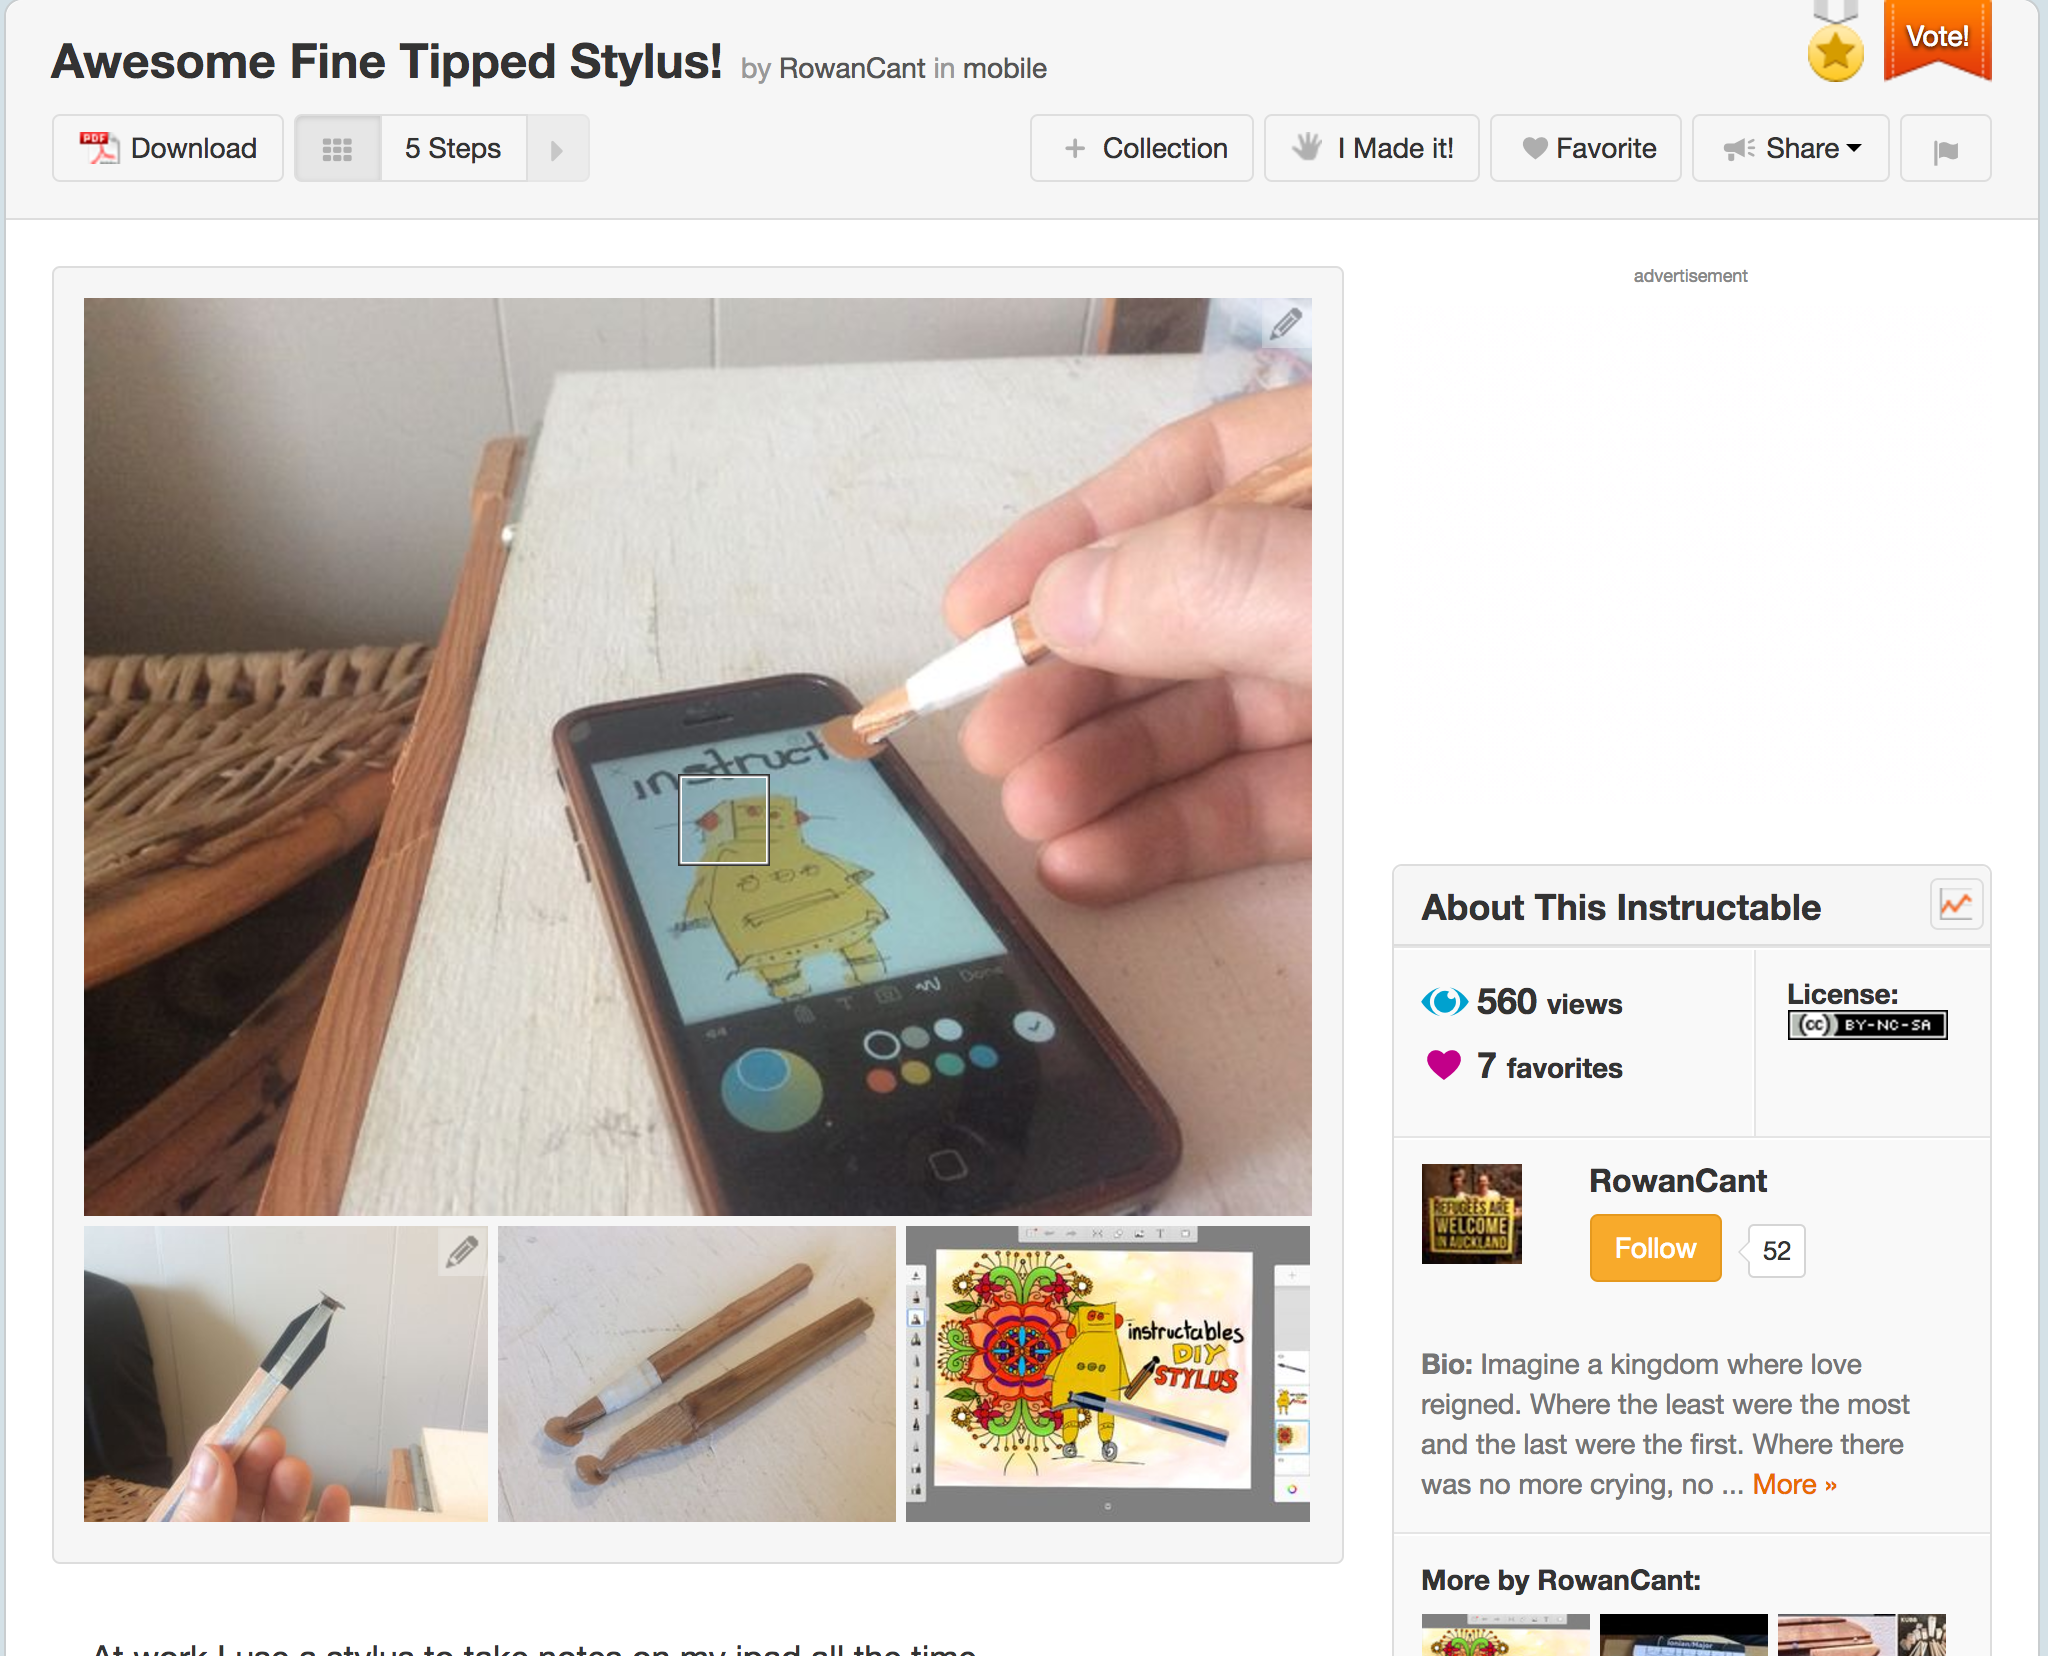
\includegraphics[scale=0.36]{./images/img-instructables.png}
	\caption{Sample Instructables project, \url{http://www.instructables.com/id/Awesome-Fine-Tipped-Stylus/}}
	\label{sec:img-instructables}
\end{figure}

Instructables is an online platform for \textit{DIY} communities that serves as a "place that lets you explore, document, and share your creations" \cite{web:instructable}. It is a website specializing in user-created and uploaded do-it-yourself projects, which other users can comment on and rate for quality \cite{wiki:instructable} \cite{wiki:instructable}. There are different categories of project such as technology, crafts, food, home, workshops and living, with more than 263,258 projects and 9,888,442 monthly visit as of August 2017. Users create their project step by step and with each step they describe what they did in a text, photos or videos as displayed in the figure \ref{sec:img-instructables}. The encapsulation of steps produce a typical guide that help others to re-create the project, learn from it or build a new thing on top of it and have their own version of the project. 

The contributions in Instructables come from the sharing culture of projects, not only authors contribute but also readers who can view and give feedback by commenting on the project. Also, Instructables create a social community where they exchange their thoughts about a topic via forums and subforms dedicated to a special topic such as Arduino projects. Finally, prizes are given to the top shared Instructables as a kind of reward for their effort of sharing their project and to keep them connected with the community.

\subsection{Methodology} 

To understand the users interactions of Instructables, an extensive study of the Instructables community has been done in the fall of 2011, this study used semi-structured interviews and online surveys. The semi-structured interviews had a framework of four themes that had been explored : (\oldstylenums{1}) motivation, (\oldstylenums{2}) Documentation tools, (\oldstylenums{3}) Writing an Instructable and (\oldstylenums{4}) Feedback. A theme was covered by a set of questions that took one hour with each interviewer. \cite{scholar:Tseng:2014:PVP:2598510.2598540}. A survey of 15 multiple-choice questions and open ended-questions that ask users about different aspects of their experience with replicating or building on top of a project shared by a user on the platform.

\subsection{User interaction}

The study has shown three strategies for documenting a project. The first was to \textit{write after you make}, as shown in the figure \ref{img-writemake}  \cite{tseng2016making}.
\begin{figure}[ht!]
	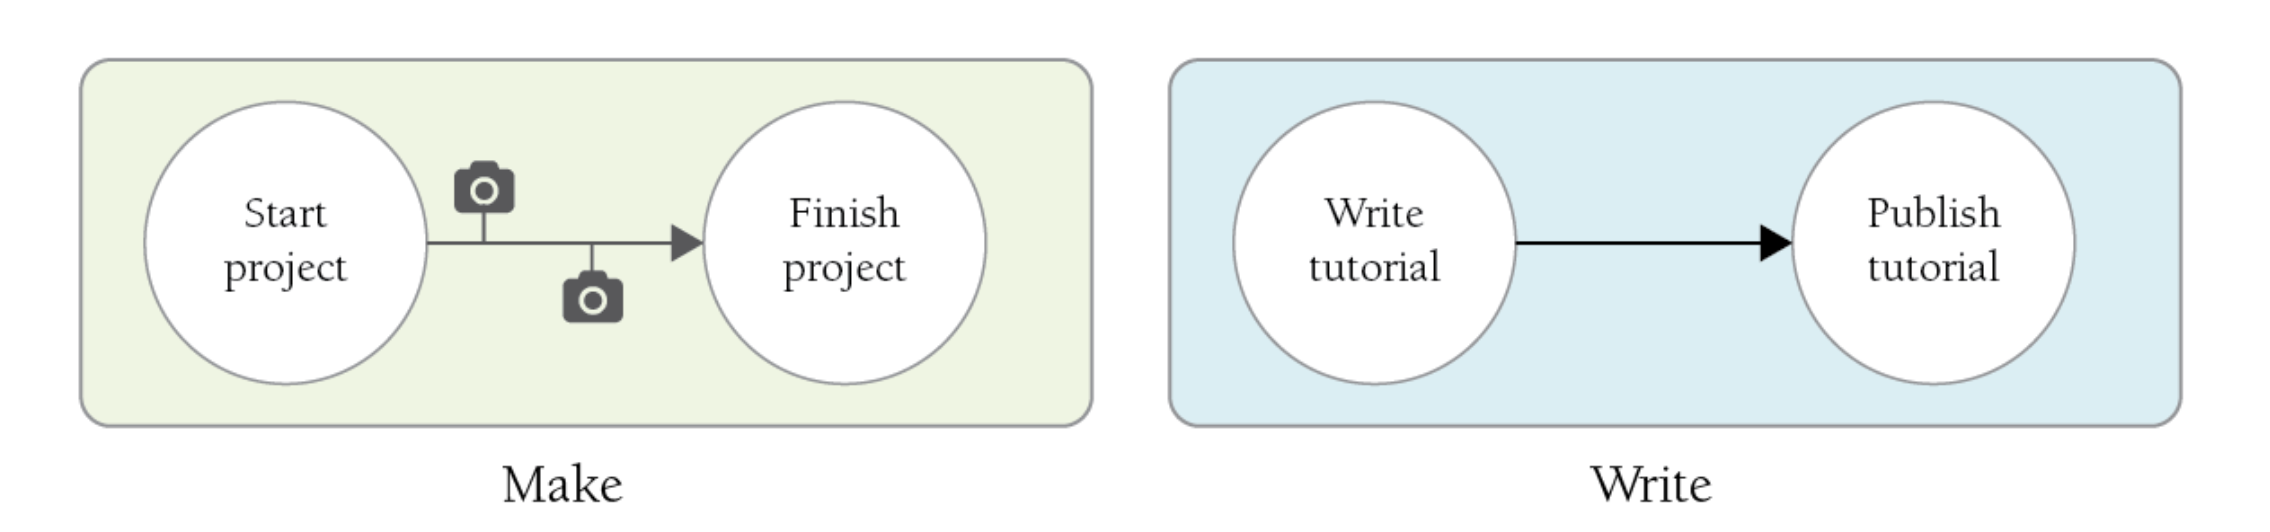
\includegraphics[scale=0.34]{./images/img-writemake.png}
	\caption{First strategy of documenting : write after you make, \cite{tseng2016making}}
	\label{img-writemake}
\end{figure}

A problem confronted the users with this strategy, users forgot to document in the midst of making. Users outperformed this problem by following the second strategy of \textit{writing after replicating}, as displayed in the figure \ref{img-makereplicatewrite} \cite{scholar:Tseng:2014:PVP:2598510.2598540}
\begin{figure}[ht!]
	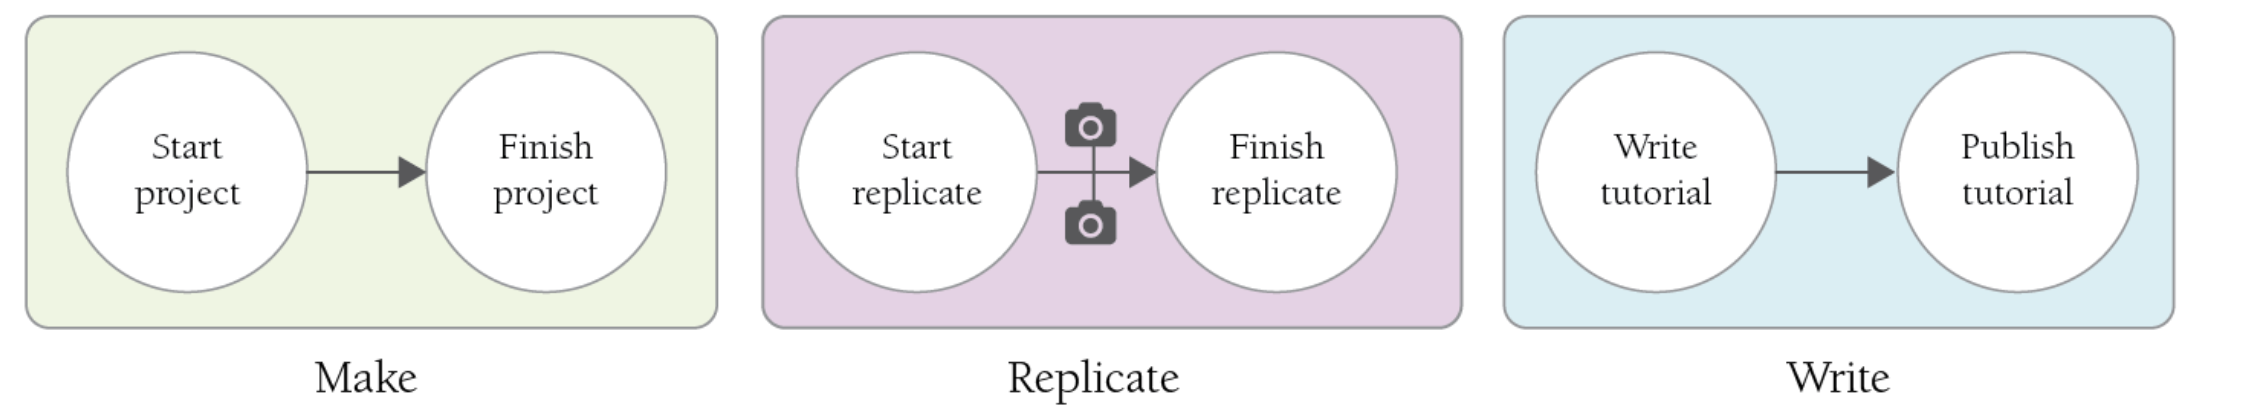
\includegraphics[scale=0.34]{./images/img-makereplicatewrite.png}
	\caption{First strategy of documenting : Make, replicate  then write, \cite{tseng2016making}}
	\label{img-makereplicatewrite}
\end{figure}

The final strategy was to \textit{simultaneously write and make} (figure \ref{img-makewritesimultanously}). 
\begin{figure}[ht!]
	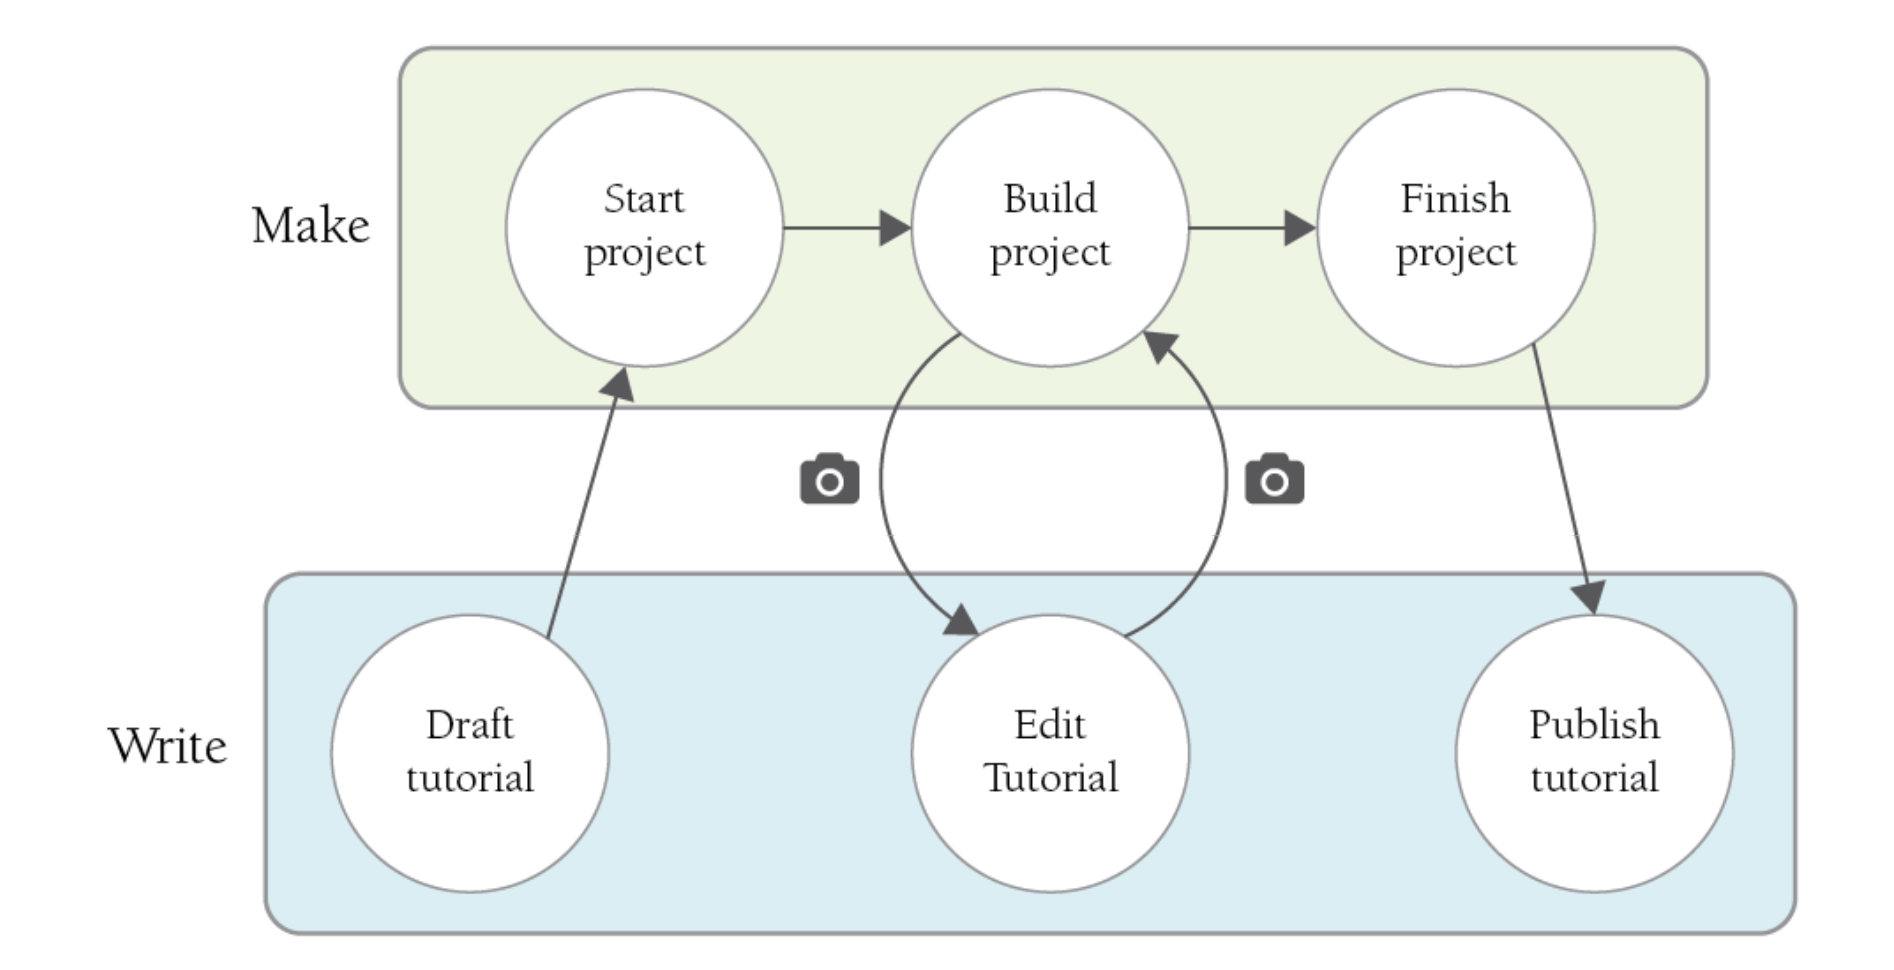
\includegraphics[scale=0.34]{./images/img-makewritesimultanously}
	\caption{First strategy of documenting : write after you make, \cite{tseng2016making}}
	\label{img-makewritesimultanously}
\end{figure}

In summary, the study showed that users need to encapsulate the collected photos and videos to show to create all the steps and a common challenge was to remember to document after each step otherwise users had to replicate their project merely to creating good documentation. 

Finally, authors saw that documentation well worth the effort to share their work but it is time consuming process when a project get more complex, it is hard to follow up or complete the documentation. \cite{scholar:Wakkary:2015:TAH:2702123.2702550}

\subsection{Design and process oriented documentation}
Several approaches were suggested by to improve the online documentation. Documentation techniques requires authors to simultaneously switch between making and writing, make a design process to not miss a step from not being documented or to radically recreate the project to document it in a proper way. Another challenges of documentation technique that needed to support not only the capture of digital artifacts but also physical artifacts where it is not possible to show the physical effort. 
With the recurring need to balance manual and automated ways of capturing, software and hardware tools need to solve open questions and be customizable for different activities and different audiences \cite{Kuznetsov:2010:REA:1868914.1868950}. The workflow of documentation over time needed to not miss a key step in the documentation. 

Documentation process seems to be more important for readers as it give them the opportunity to enable better decision making about components or materials to use \cite{scholar:sf1241364}, as well as successful in encouraging independent exploration and fostering a sense of accomplishment \cite{scholar:lovell2010sewing}. Also, as many users start by replicating some projects, having tools where they could be able to contribute to a project, can help more socializing and boost a collaborative work in the community. 

\section{Build In Progress}
%\hl{What is it ?} \hl{Who use it ?} \hl{User interactions ?} \hl{Limitations} \hl{Advantages ?} \hl{Examples ?}

Build in Progress is a platform for sharing the story of your design process, where \textit{"makers share how their DIY projects evolve over time}" \cite{tseng2016making}. It focus more on the storytelling of \textit{DIY} documented project, a snapshot of the platform displayed in the figure \ref{img-buildinprogress}.

BiP was launched in 2013 and within a collaboration with many institutions and a network of schools, it hosted over 1368 projects in categories such as Electronics, Mechanical and living. Users contributed to BiP community by sharing, providing feedback and describing their progress of each step, the encapsulation of informations lead to a story about the project as BiP "\textit{support a storytelling approach to documentation}" \cite{tseng2016making}.
\begin{figure}[ht!]
	\centering
	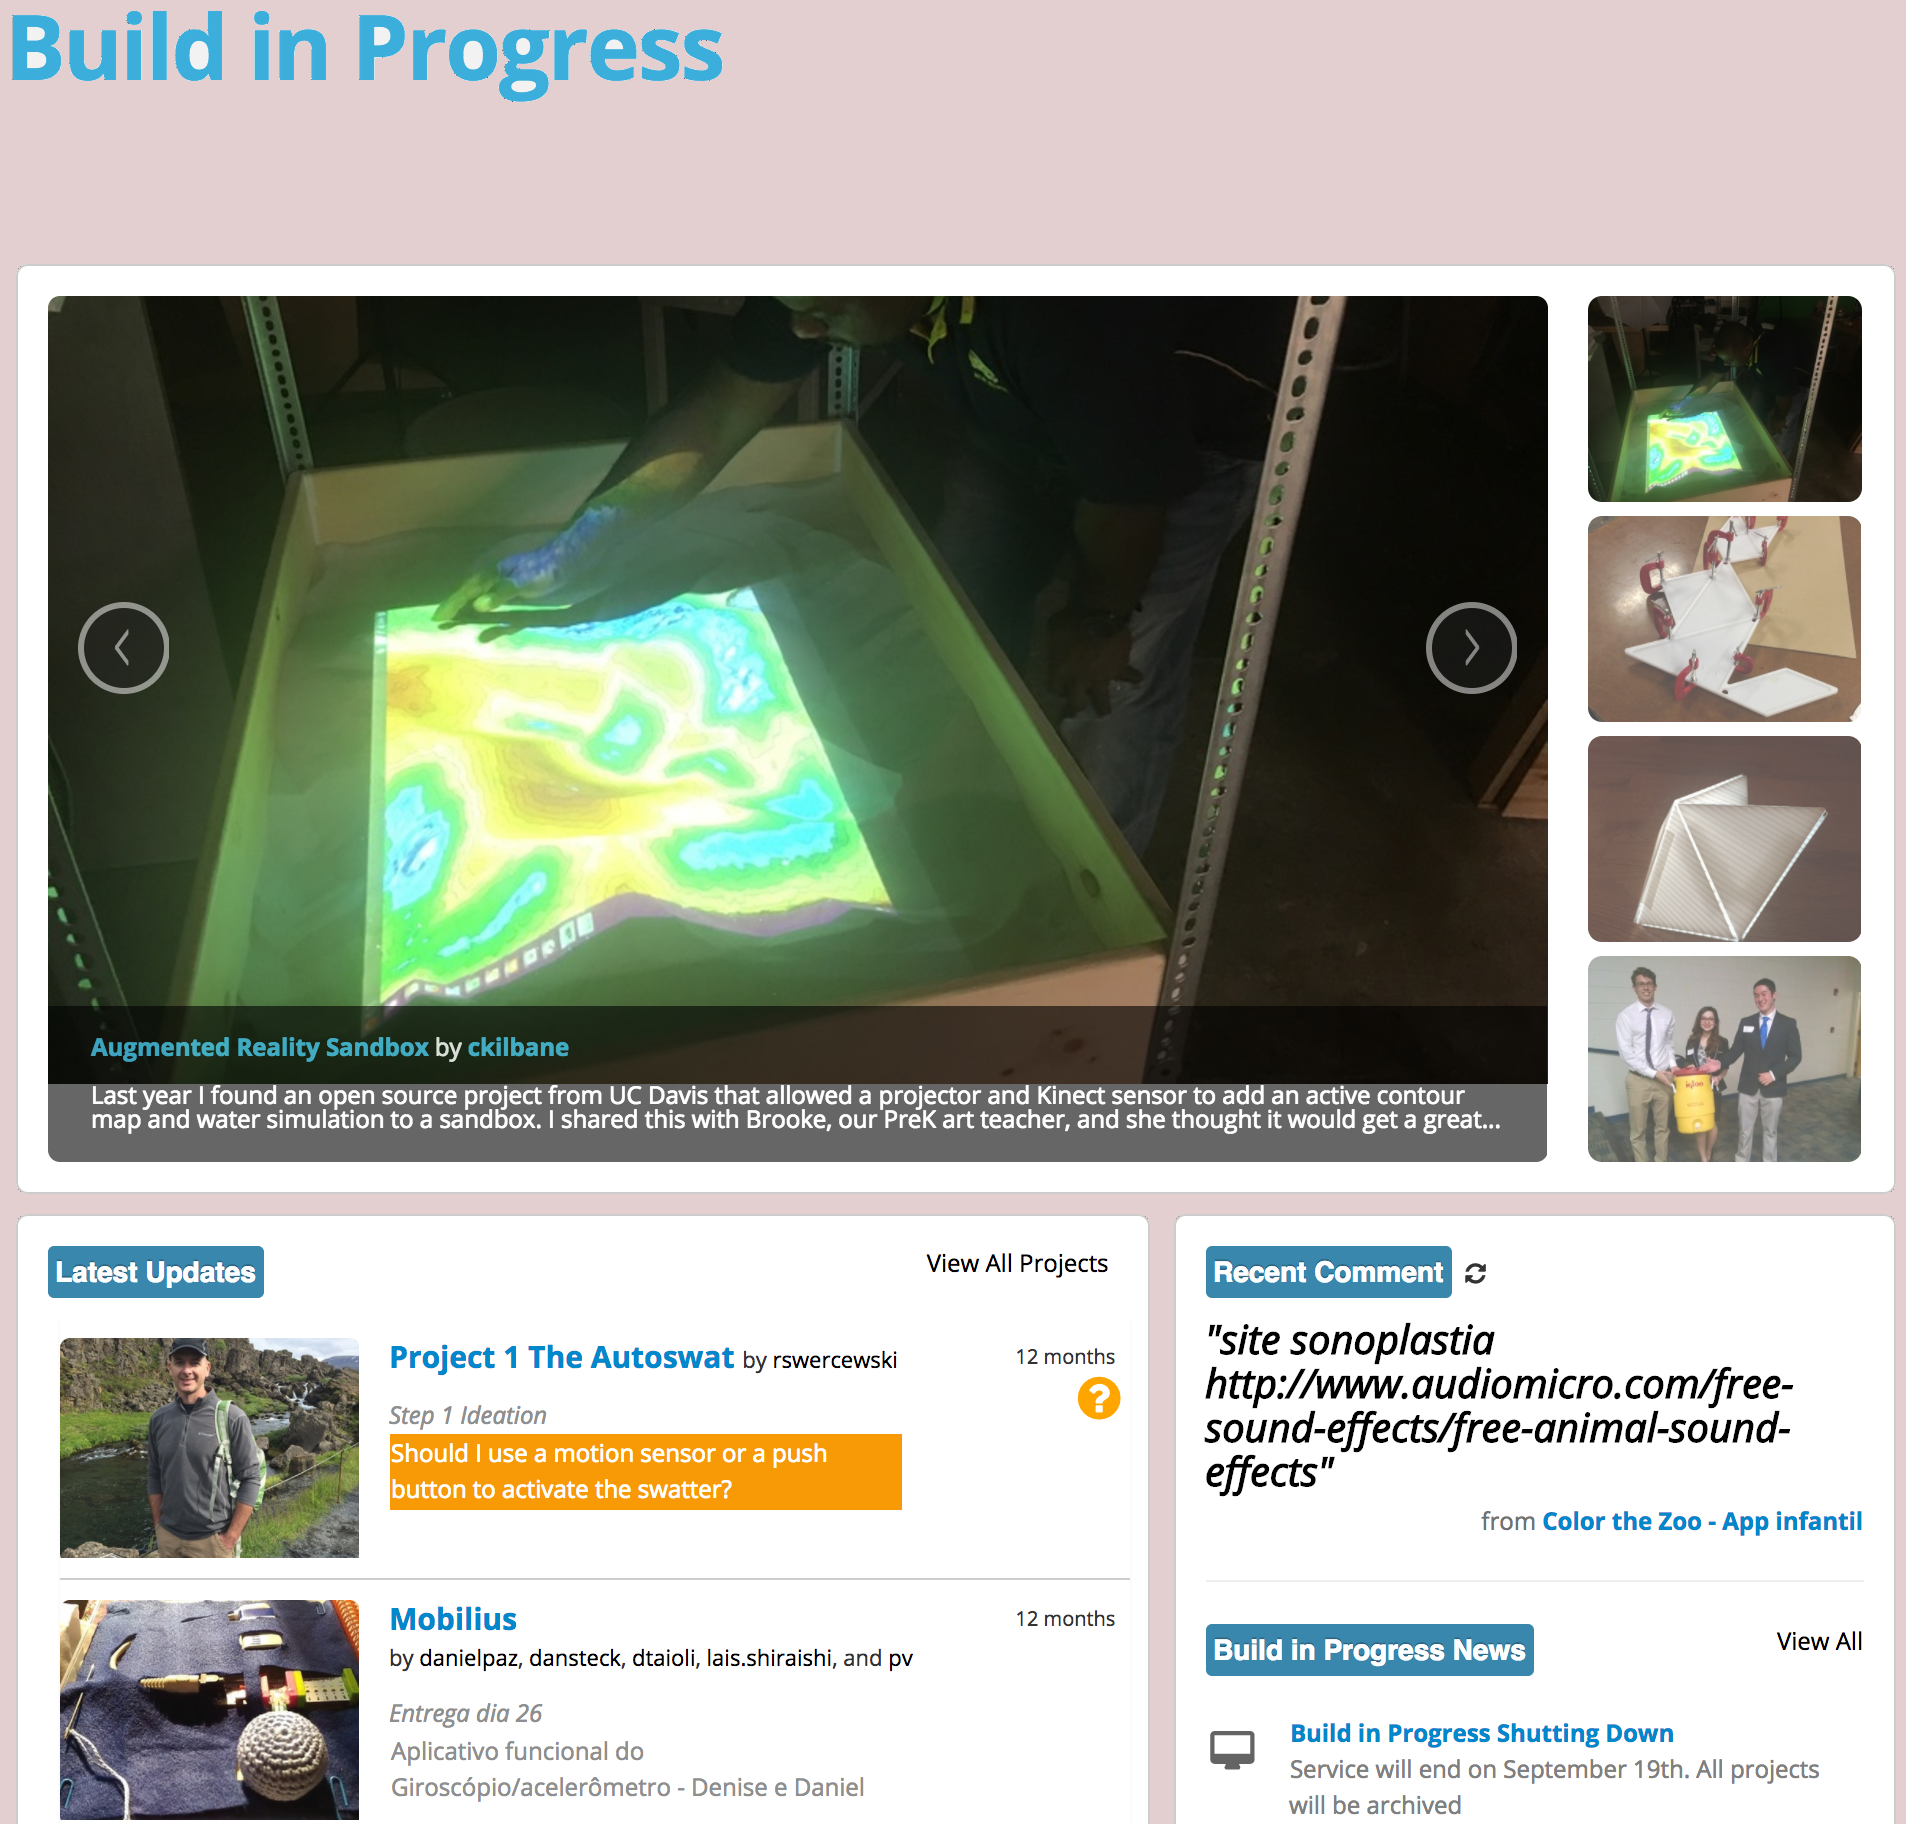
\includegraphics[width=10cm, height=10cm]{./images/img-buildinprogress.png}
	\caption{Build in progress welcome page, \cite{BuildinP1}} 
	\label{img-buildinprogress}
\end{figure}

\vspace{-1cm}
\subsection{Design approach}
Authors shared an iterative design process in the context of sharing their personal journey by creating step-by-step instructions of their project via the online platform \textit{BiP} and companion mobile application. Readers contributed by suggesting to makers after publishing their steps, makers benefited from sharing step-by-step instructions over time by taking into account the suggestions of readers.

BiP was developed based on an innovative design process, it enables users to visualize their documentation in an iterative way. Authors can continuously iterate their building process, share their techniques to help others to reach out others in the community so they can have feedback. A social design process principle was considered among the online community to engage users more, to accumulate knowledge, to learn from others and connect users with same interest as \textit{human-related issues in the form of social ties and knowledge sharing were reported as keys to successful collaboration} \cite{Kotlarsky2005}.

\subsection{Features}\label{sec:feature}
BiP consists of many features in the project page and social feature. The two core features of the project page are : the \textit{Process Map} and \textit{Step Detail View } (\ref{img-bipprojectpage}).
\begin{figure}[ht!]
	\centering
	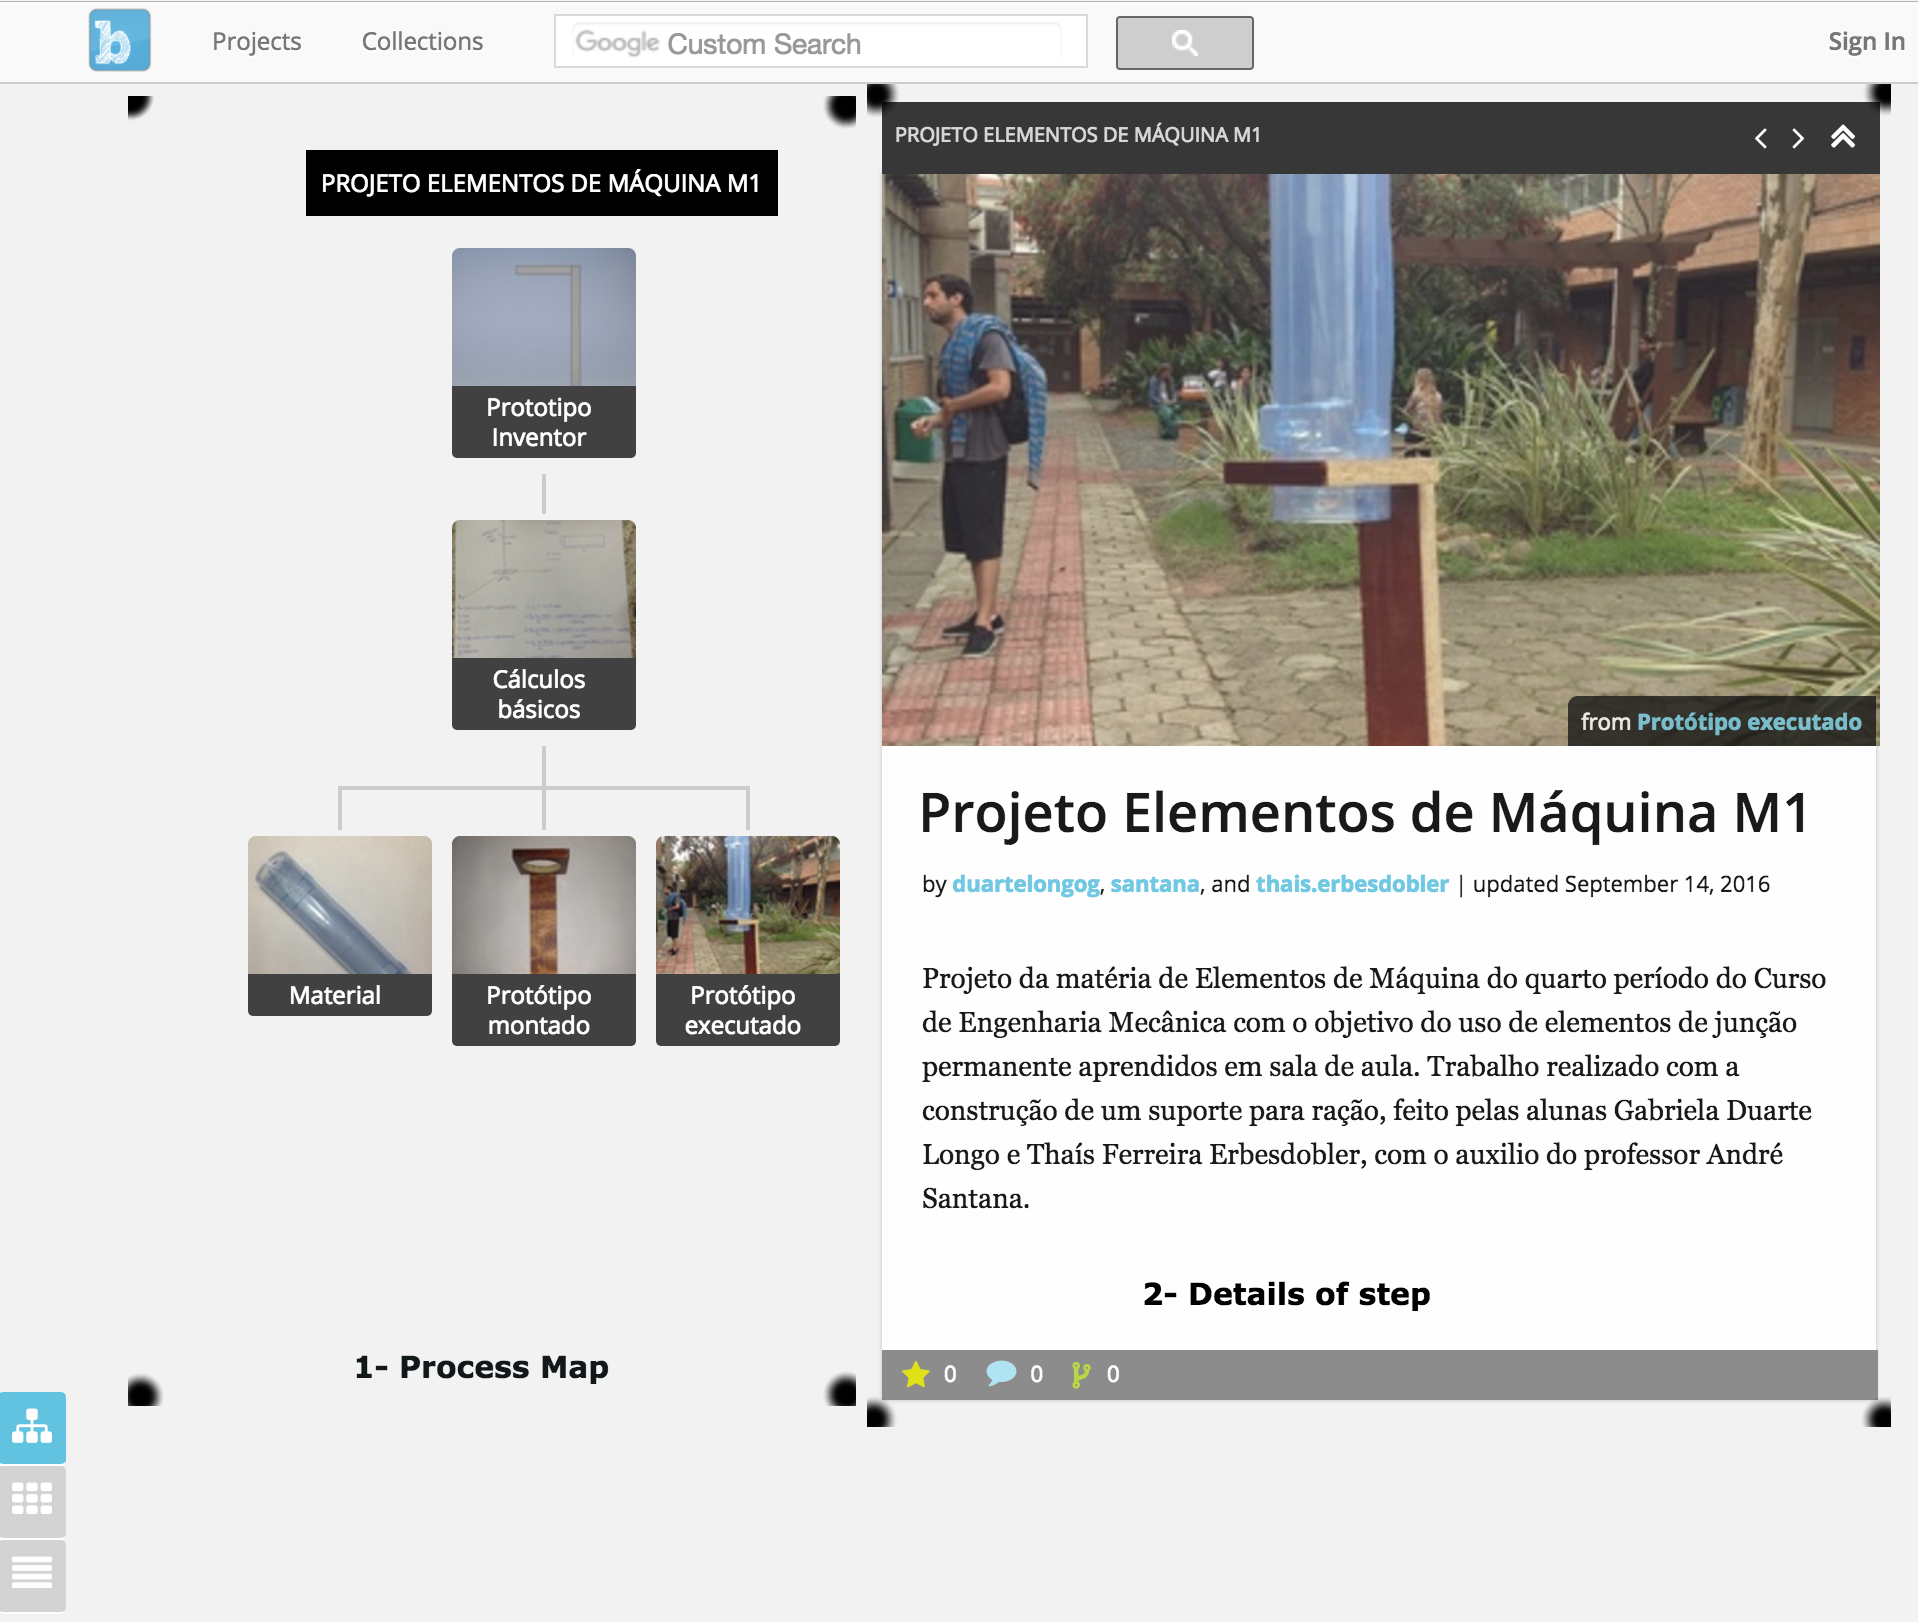
\includegraphics[width=.3\textheight]{./images/img-bipprojectpage.png}
	\caption{overall project view, \cite[\url{http://buildinprogress.media.mit.edu/projects/4599/steps}]{BuildinP2}} 
	\label{img-bipprojectpage}
\end{figure}
In the process map, users can create a step, a label for one or more step, drag \& drop  to rearrange steps. Steps are organized in a tree-map-like format with sui generis branches, a label is added to a branch and it can be colored to designate a branch; for example orange labels represent that a branch is in progress.

Project are displayed in 3 different mode.  The first is the default mode : tree-map, users can go through all the steps, step-by-step and discover more about it as shown in figure \ref{img-mode1}.
\begin{figure}[H]
	\centering
	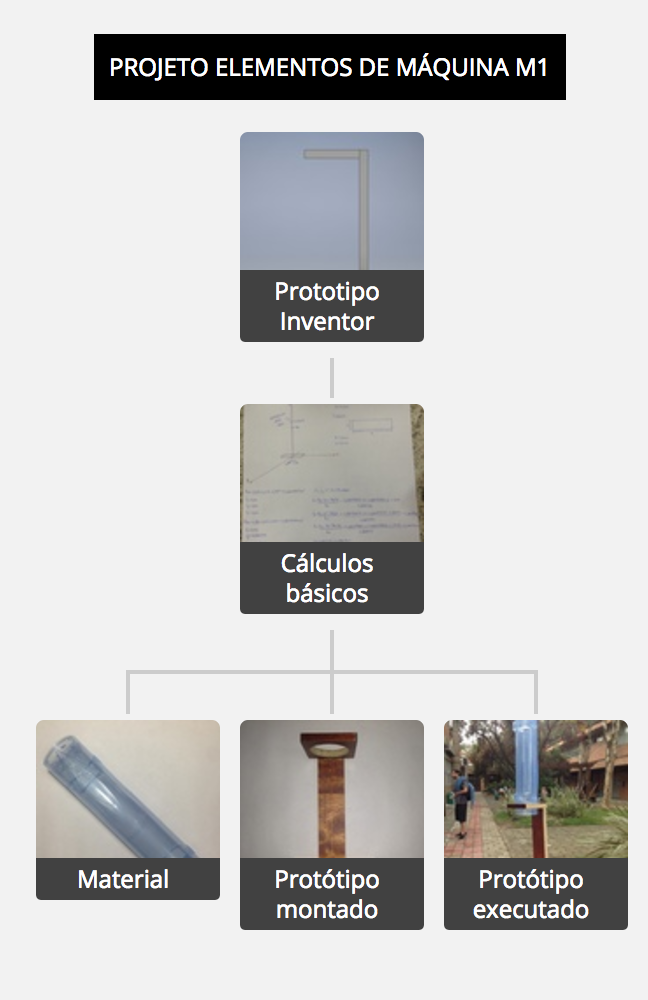
\includegraphics[scale=.3]{./images/img-mode1.png}
	\caption{tree-map view of the project} 
	\label{img-mode1}
\end{figure}

The second is Gallery mode \ref{img-mode2} and finally  the  blog mode : users can scroll down and an index of steps will be displayed on their left side of the page (figure \ref{img-mode3}).

\begin{figure}[H]
	\centering
	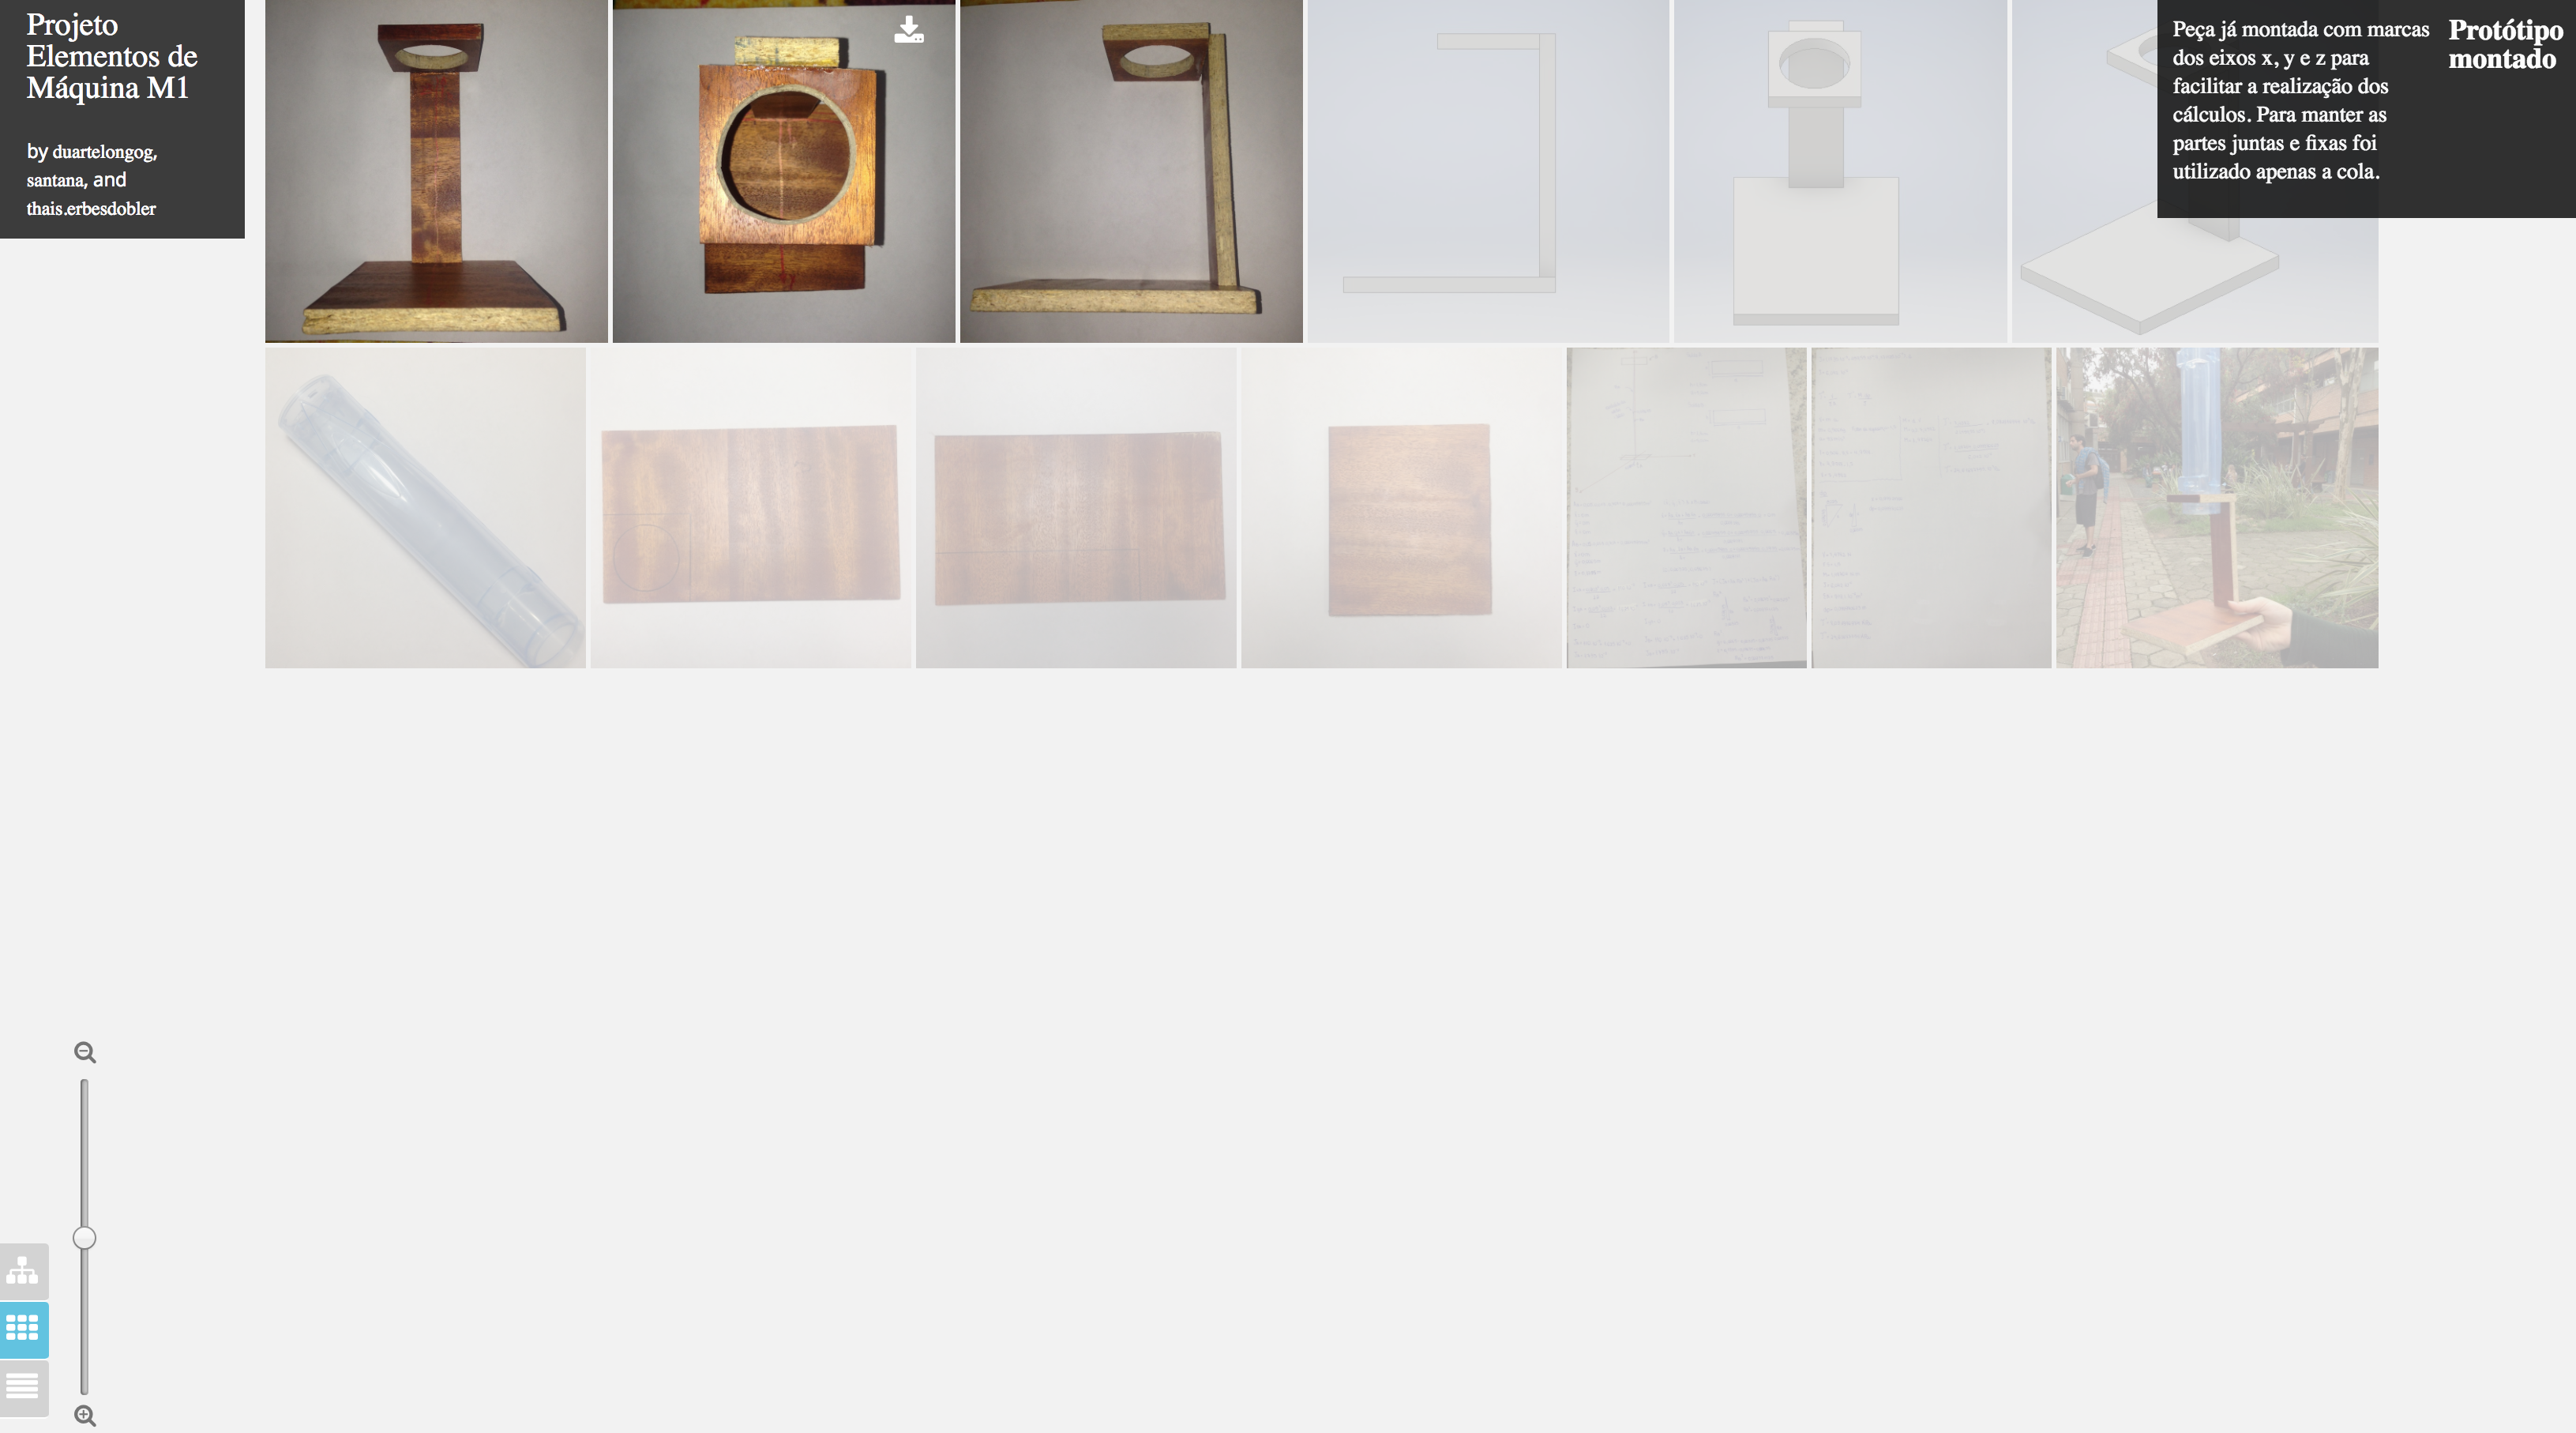
\includegraphics[scale=.16]{./images/img-mode2.png}
	\caption{Gallery view of the project} 
	\label{img-mode2}
\end{figure}

\begin{figure}[H]
	\centering
	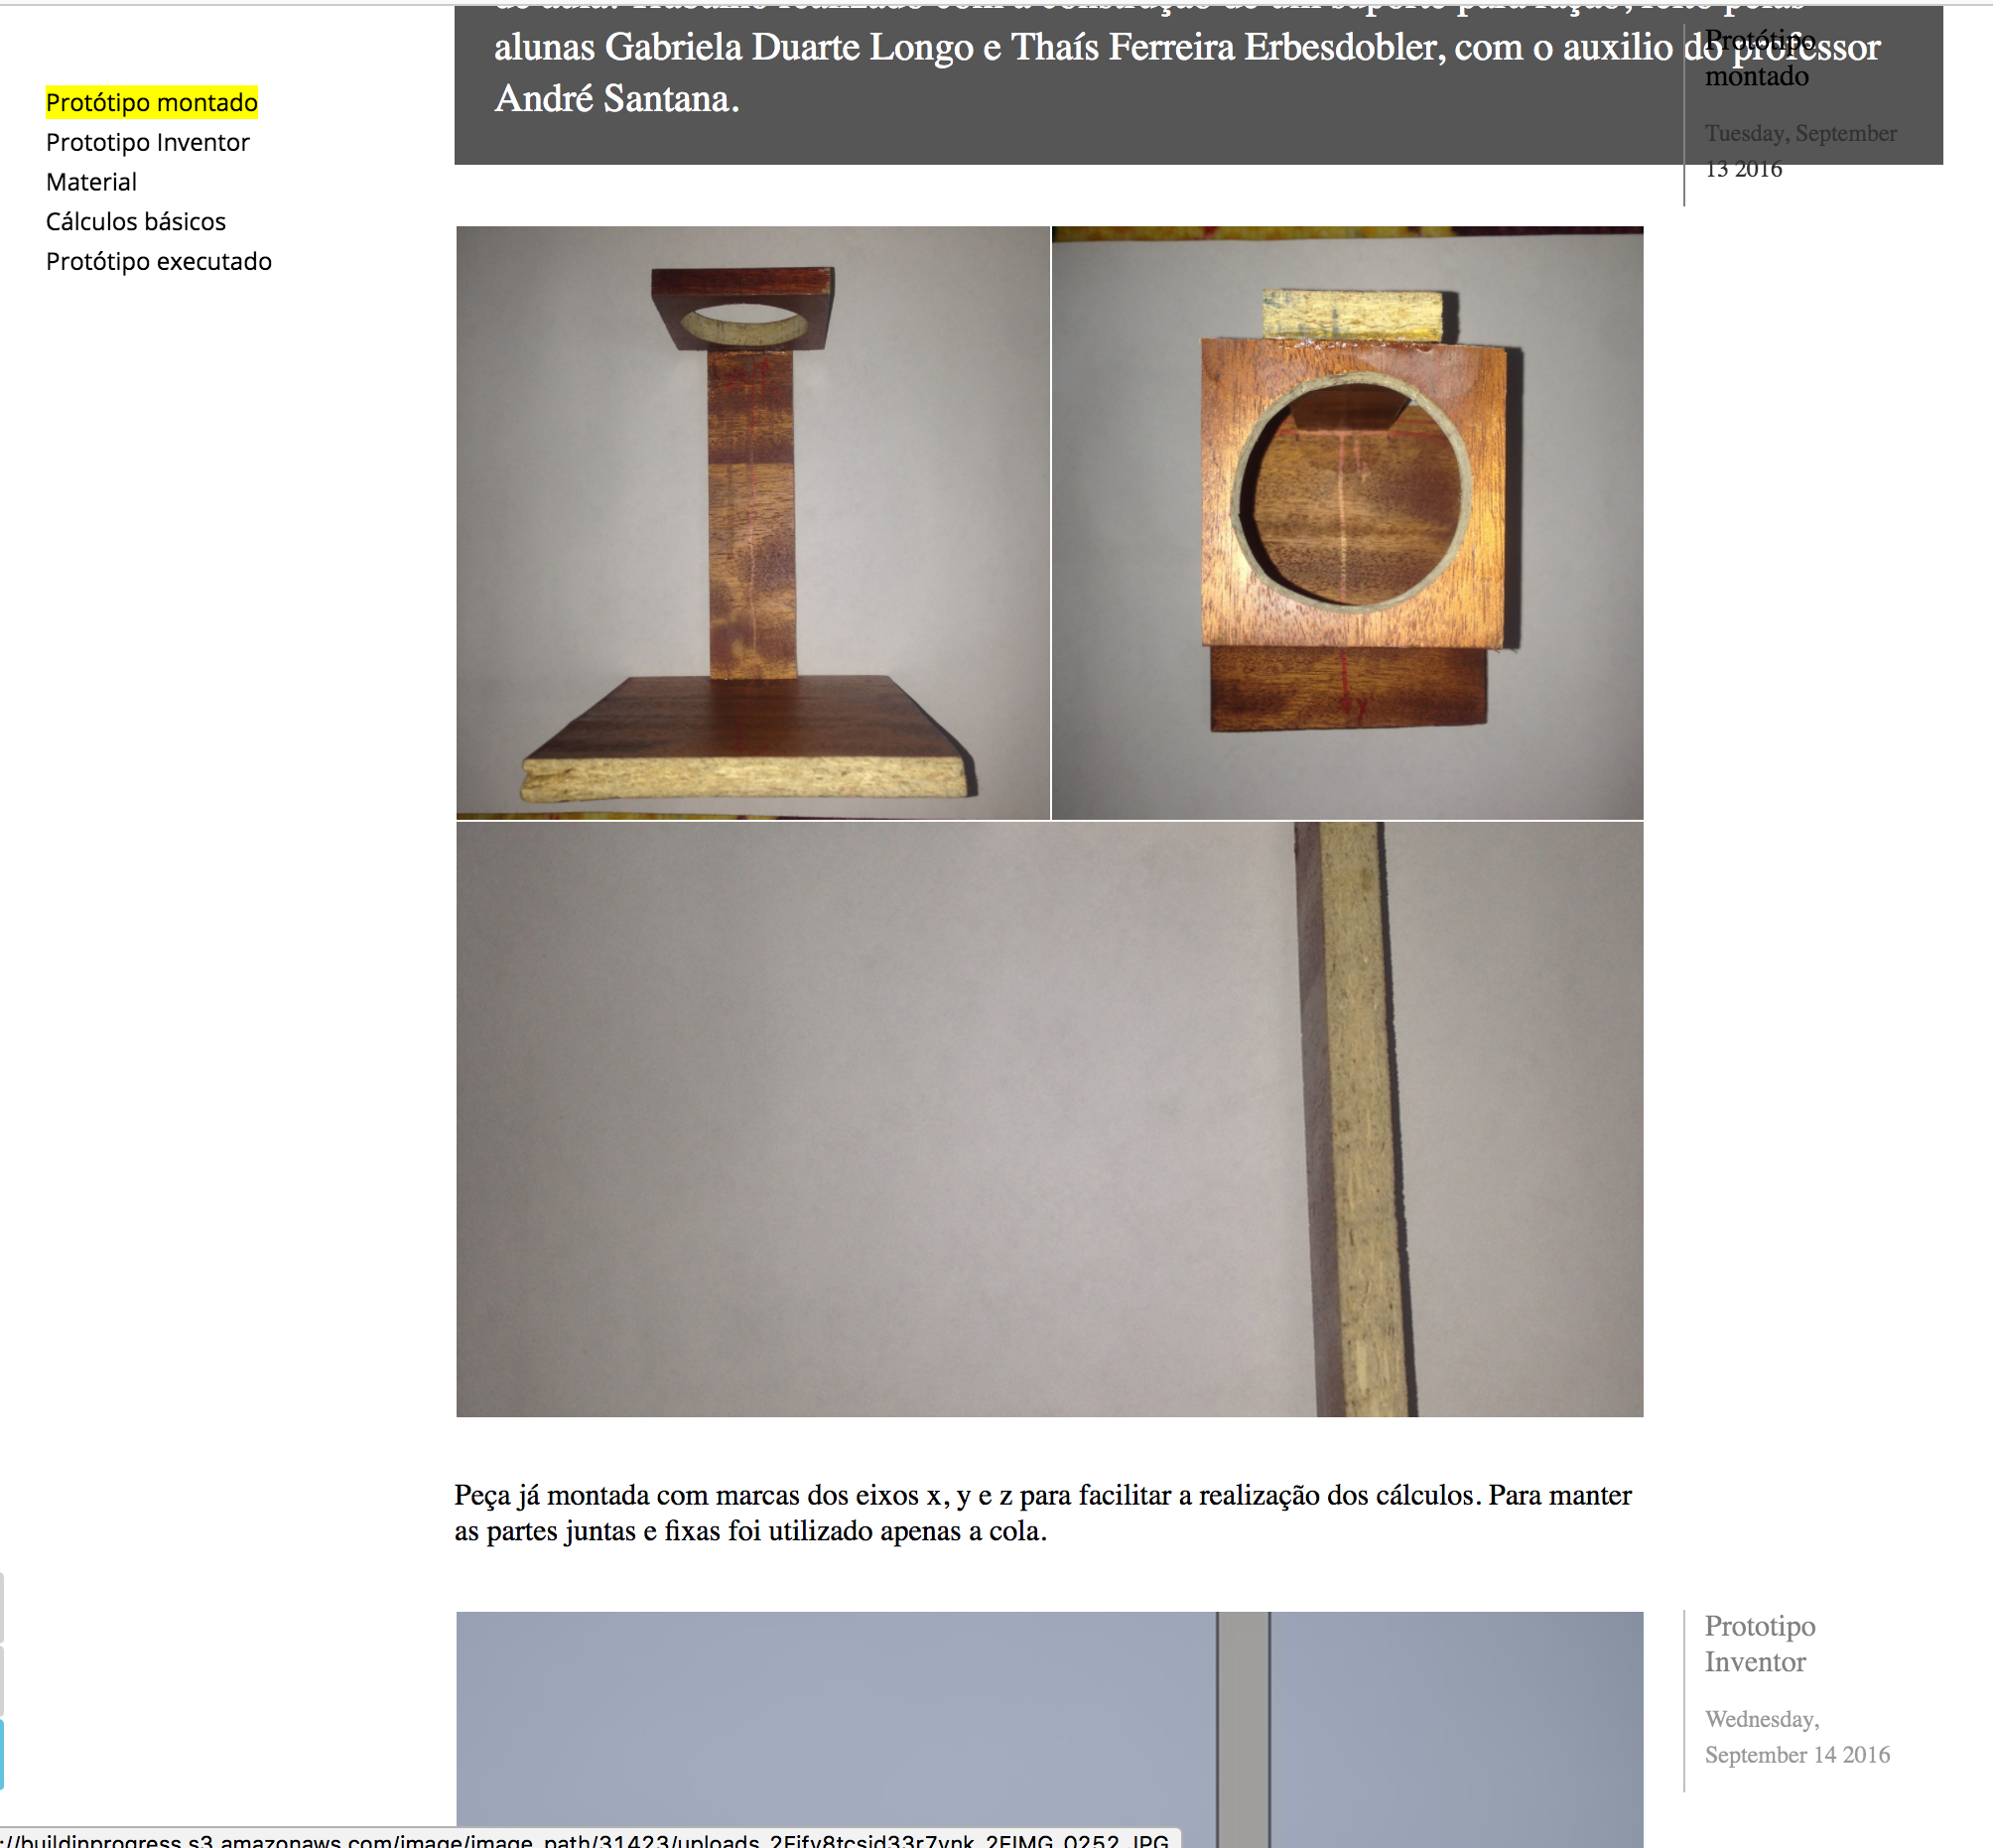
\includegraphics[scale=.3]{./images/img-mode3.png}
	\caption{Blog like mode} 
	\label{img-mode3}
\end{figure}

In \textit{Details of step} users can upload photos or videos, add text description, ask others a question that will appear in the homepage of the platform, upload resources or files in different formats; e.g. .PDF, .PPT, a given example is shown in the figure \ref{img-stepdetails} .
\begin{figure}[H]
	\centering
	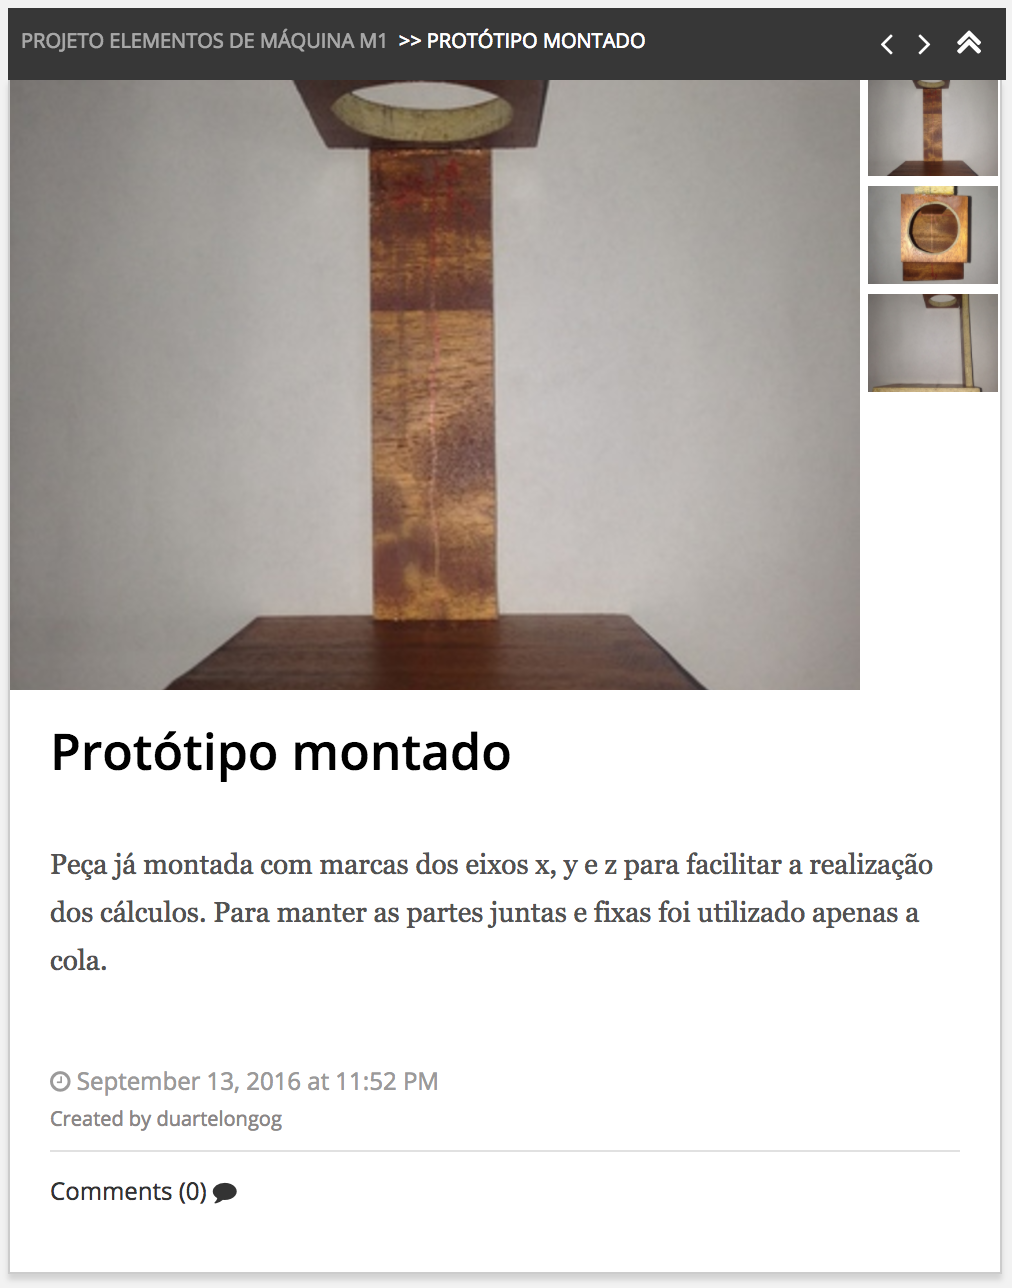
\includegraphics[scale=.3]{./images/img-stepdetails.png}
	\caption{Details steps view} 
	\label{img-stepdetails}
\end{figure}

The online platform incorporate many features that keep the BiP community more socialized and connected. Users can follow a project, see recent activity on the homepage and they will receive notification once an author add a step or ask a question.
\begin{figure}[H]
	\centering
	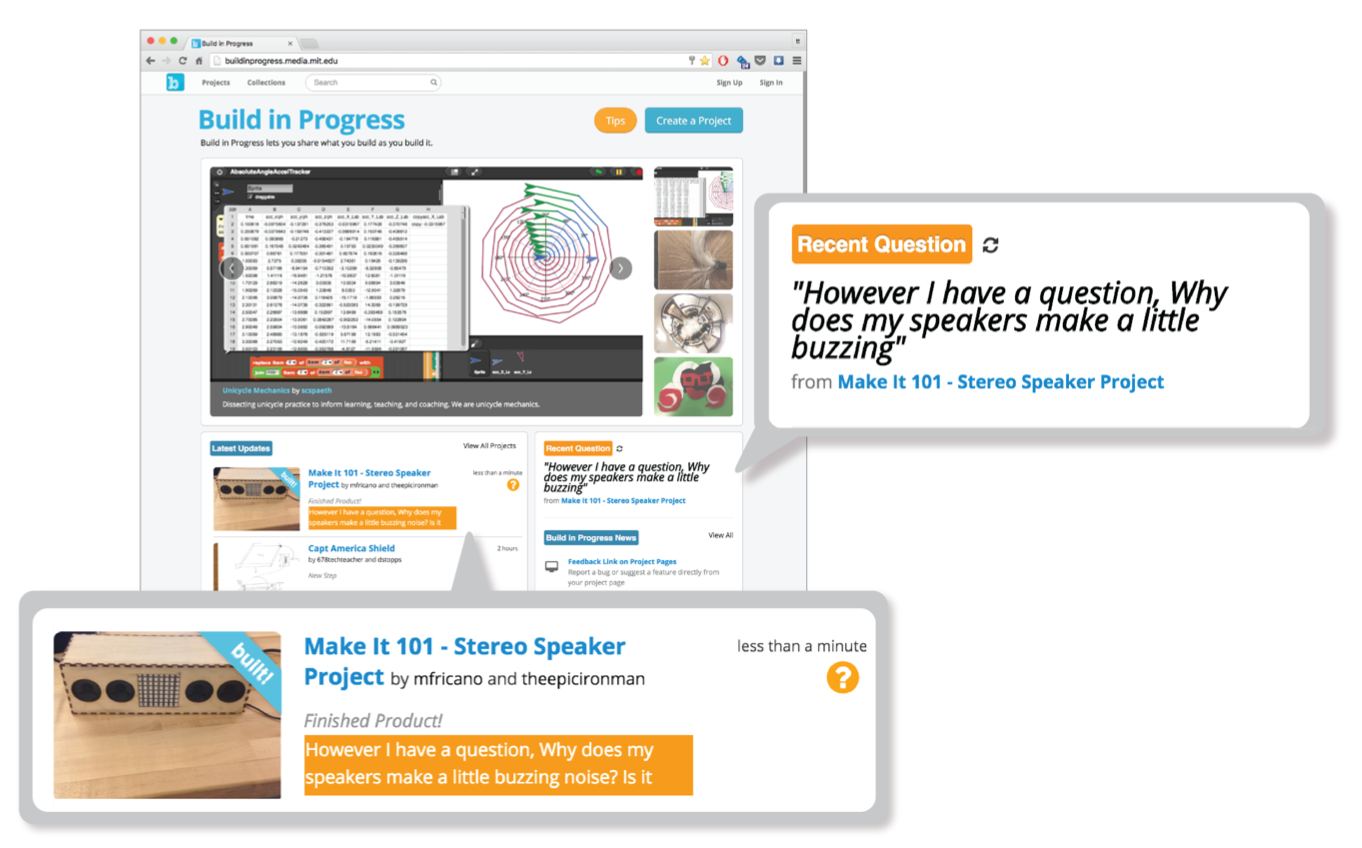
\includegraphics[scale=.4]{./images/img-commentquestion.png}
	\caption{Question featured in the home page, [Tseng, 2016]} 
	\label{img-commentquestion}
\end{figure}

Moreover, users can leave a text on any step and they will receive a notification when a comment is left. Authors can ask for feedback or help by embedding a question that will be added to the Community Activity section of the homepage, see figure \ref{img-commentquestion}.
\subsubsection{Mobile application}
A mobile application has been created to make documentation more efficient in which users upload images and videos to their projects directly from their devices instead of taking picture from their devices then transfer it to a computer and upload it (figure \ref{img-mobileapp}.
\begin{figure}[H]
	\centering
	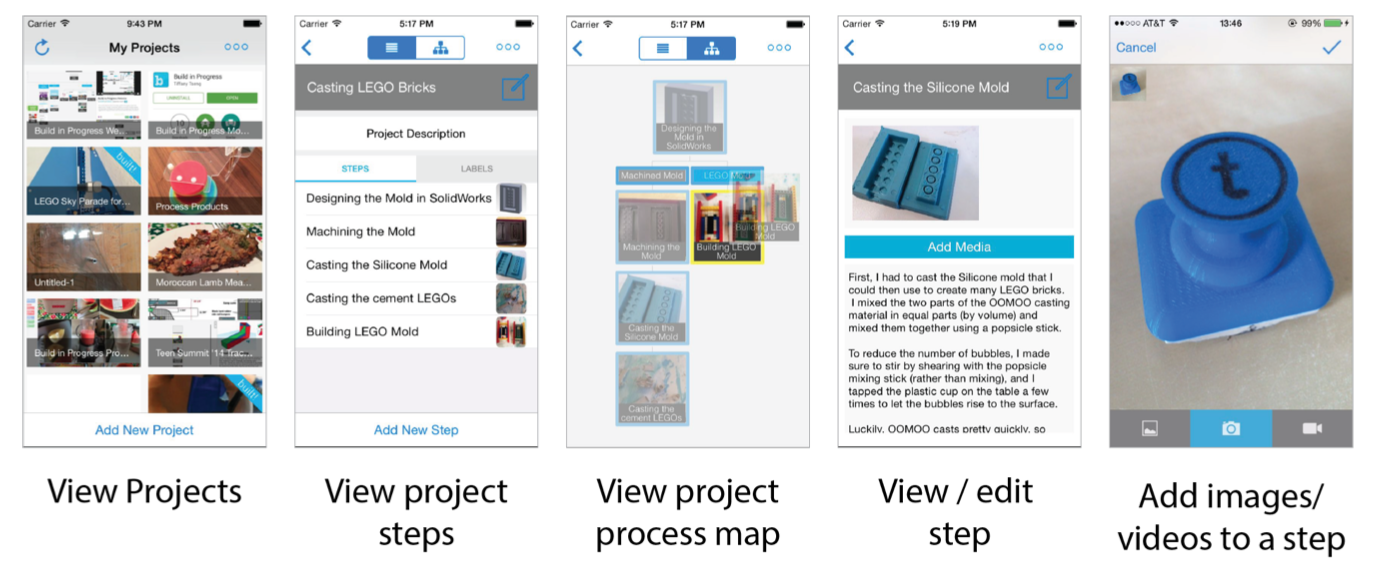
\includegraphics[scale=.5]{./images/img-mobileapp.png}
	\caption{Mobile application interface, [Tseng, 2016]} 
	\label{img-mobileapp}
\end{figure}
\subsection{User interaction}

BiP has been used in after-school  programs, in school and in workshop challenges by students and makers who work on their own project. Teenagers and one adult facilitator have been interviewed and a weekly survey was sent to all users to get an estimation about their weekly hours work.

The results of the interviews and surveys showed that users get motivated to share their project as it facilitate getting feedback, create and show their portfolio projects, get engaged to document and to help others. Users found that BiP support meaningful documentation practices and many strategies were identified depending on the type of project, the duration of a project and the age of makers who are using it.

\subsection{Summary}

The study of BuildinProgress showed that BiP support authors and readers. The documentation help makers to create a design process for their project by learning from the many iterations they did over time and BiP motivates reflective practice on making, design process, and values and identity. Users get engaged, get feedback, get self reward and help others. It support all capturing way written and visual. 



\section{Discussion}

\textit{BuildinProgress} and \textit{Instructables} didn't bring a new fundamental way in which users can share their captured media publicly or in private. Design parameters can be adjusted to support different type of users-interactions and goals.  Instructables enable users to personalize through substitution and modification of a step and any missing step mean that authors should re-create their documentation while BiP focus more on the  design process where users can iterate their project by creating new branches and forget about the unsuccessful branches.

The mix between capturing and text-based-description features in BiP enable teenagers to document. The ease of use for creating a branch, drag \& drop simplify the job for younger audience especially readers who are new to the community of \textit{DIY} as they can go through steps, iterate on their work, modify a step or re-arrange some steps.  Instructables has both features but there is no friendly structure where authors get their documentation organized and if an author has a limited background in documentation or he doesn't like it, he will probably abandon the documentation of a project after the first type a user find that it is not possible to re-arrage the documented steps.

Sharing a project is not enough for authors. Users in Instructables found that they cannot share their thought or it is limited as the only way to express what they think is via a comment. BiP offers a text-based option where both authors and readers could ask a question or leave a comment, also, both can receive a notifications for a reply from the community or any other news concerning any modification in the project.

The process of sharing the effort in progress enable users to communicate more in BiP, they helped each other, they showed their effort, they get featured and receive feedback as described in section \ref{sec:feature}. Balancing the ease of use of automated documentation systems with the powerful feature, a mobile application, encourage more users to upload pictures or videos and enable them to be physically free so they can move around to document their project for example without having the problem of taking a photo, remember which step it is, transfer it then upload it to the platform as in Instructables.

\section{Conclusion \& Future Work}

As we see, innovators need tools of documentation to support their innovations. I found that one tool is not enough to support different goals and types of interactions especially if users are from different background and ages. But the availability of features in some tools can enable users to fulfil their need either in showing their effort, keep tracks of their ideas, sharing their experience or exchange knowledge \cite{doi:10.1287/orsc.1070.0325}. 

In this state-of-the-art I analysed \textit{Instructables} the most popular online community for \textit{DIY} and the most recent \textit{DIY} platform \textit{BuildinProgress} but at the same time I went through many other online community \textit{Dorkbot, Ravelry, Craftster, Etsy, hacker, hackster.io} and I found that \textit{DIY} community share one need : A tool that enable makers, hackers and innovators to share their experiences in  a proper and meaningful ways.  Another thing I have learned from my experience of more than 13 hackathons, the analyses of \textit{Instructables}  and \textit{BiP} is that developing a new tools will not bring a new fundamental way of capturing media or writing text for documentation. Eventually, a goal would be to improve the process map used in BiP. 

I can conclude that an existing tool is needed from a wide range of \textit{DIY} community that would enable them to document in a meaningful way and make their documentation more sustainable. I believe, a tool that contains all necessary features for documentation with enhanced design process could be the new popular tool to use by \textit{DIY} community to document their effort in meaningful ways. To prove this we need to see how hackers, makers and innovators will use this tool, how useful is it and the method of design process would be questioned.


\begin{comment}

\begin{itemize}
	\item{Adapt  SDG in progress}
	
	
	\item{Qu-est ce que la platforme a apporte et ce que nous on a apporte}
	\item{Comparaison avec other platform}
	\item{ Explication about the summer school, experience, different way to document etc..} 
	\item{When we can use it and how we can use it ?} 
	
\end{itemize}


\begin{itemize}
	\item Platforme pour le soutien des hackathon grise
	\item What tiffanz said about here ieda and references
	\item securite constructif
	
	\begin{itemize}
		\item la continuite des  idess
		\item durabilitz of projects
		\item relance les projet
	\end{itemize}
	\item hackathons
	\item summer school
	\item master
	\item how to evaluate a project in time when it avaluate from team to team
	\item changement de step ou de team, continuite sachant qu'on connait des interruption forte , d'etape, d'equipe, et les 2 rests ensemble
	\item cumulative innovation
	\item in innnovation find a waz to document goodlz 
	\item rice made
	\item 
\end{itemize}

\section{IDEAS}
\begin{itemize}
	\item "Users don't want documentation, they want answers" 
\end{itemize}

\section{Features}

%% This is an example first chapter.  You should put chapter/appendix that you
%% write into a separate file, and add a line \include{yourfilename} to
%% main.tex, where `yourfilename.tex' is the name of the chapter/appendix file.
%% You can process specific files by typing their names in at the 
%% \files=
%% prompt when you run the file main.tex through LaTeX.




\label{sec:features}

The rest of this document shows off a few features of the template
files.  Look at the source code to see which macros we used!

The template is divided into \TeX{} files as follows:
\begin{enumerate}
\item \texttt{thesis.tex} is the main file.
\item \texttt{extrapackages.tex} holds extra package includes.
\item \texttt{layoutsetup.tex} defines the style used in this document.
\item \texttt{theoremsetup.tex} declares the theorem-like environments.
\item \texttt{macrosetup.tex} defines extra macros that you may find
useful.
\item \texttt{introduction.tex} contains this text.
\item \texttt{sections.tex} is a quick demo of each sectioning level
available.
\item \texttt{refs.bib} is an example bibliography file.  You can use
Bib\TeX{} to quote references.  For example, read
\cite{bringhurst1996ets} if you can get a hold of it.
\end{enumerate}


\subsection{Extra package includes}

The file \texttt{extrapackages.tex} lists some packages that usually
come in handy.  Simply have a look at the source code.  We have
added the following comments based on our experiences:
\begin{description}
\item[REC] This package is recommended.
\item[OPT] This package is optional.  It usually solves a specific
problem in a clever way.
\item[ADV] This package is for the advanced user, but solves a problem
frequent enough that we mention it. Consult the package's
documentation.
\end{description}

As a small example, here is a reference to the Section \emph{Features}
typeset with the recommended \package{varioref} package:
\begin{quote}
See Section~\vref{sec:features}.
\end{quote}


\subsection{Layout setup}

This defines the overall look of the document -- for example, it
changes the chapter and section heading appearance.  We consider this
a `do not touch' area.  Take a look at the excellent \emph{Memoir}
documentation before changing it.

In fact, take a look at the excellent \emph{Memoir} documentation,
full stop.


\subsection{Theorem setup}

This file defines a bunch of theorem-like environments.

\begin{theorem}
An example theorem.
\end{theorem}

\begin{proof}
Proof text goes here.
\end{proof}

Note that the q.e.d.\ symbol moves to the correct place automatically
if you end the proof with an \texttt{enumerate} or
\texttt{displaymath}.  You do not need to use \verb-\qedhere- as with
\package{amsthm}.

\begin{theorem}[Some Famous Guy]
Another example theorem.
\end{theorem}

\begin{proof}
This proof
\begin{enumerate}
\item ends in an enumerate.
\end{enumerate}
\end{proof}

\begin{proposition}
Note that all theorem-like environments are by default numbered on
the same counter.
\end{proposition}

\begin{proof}
This proof ends in a display like so:
\begin{displaymath}
f(x) = x^2.
\end{displaymath}
\end{proof}


\subsection{Macro setup}

For now the macro setup only shows how to define some basic macros,
and how to use a neat feature of the \package{mathtools} package:
\begin{displaymath}
\abs{a}, \quad \abs*{\frac{a}{b}}, \quad \abs[\big]{\frac{a}{b}}.
\end{displaymath}

This is version \verb-v1.4- of the template.

We assume that you found this template on our institute's website, so
we do not repeat everything stated there.  Consult the website again
for pointers to further reading about \LaTeX{}.  This chapter only
gives a brief overview of the files you are looking at.

\section{Features}
\label{sec:features}

The rest of this document shows off a few features of the template
files.  Look at the source code to see which macros we used!

The template is divided into \TeX{} files as follows:
\begin{enumerate}
\item \texttt{thesis.tex} is the main file.
\item \texttt{extrapackages.tex} holds extra package includes.
\item \texttt{layoutsetup.tex} defines the style used in this document.
\item \texttt{theoremsetup.tex} declares the theorem-like environments.
\item \texttt{macrosetup.tex} defines extra macros that you may find
useful.
\item \texttt{introduction.tex} contains this text.
\item \texttt{sections.tex} is a quick demo of each sectioning level
available.
\item \texttt{refs.bib} is an example bibliography file.  You can use
Bib\TeX{} to quote references.  For example, read
\cite{bringhurst1996ets} if you can get a hold of it.
\end{enumerate}


\subsection{Extra package includes}

The file \texttt{extrapackages.tex} lists some packages that usually
come in handy.  Simply have a look at the source code.  We have
added the following comments based on our experiences:
\begin{description}
\item[REC] This package is recommended.
\item[OPT] This package is optional.  It usually solves a specific
problem in a clever way.
\item[ADV] This package is for the advanced user, but solves a problem
frequent enough that we mention it. Consult the package's
documentation.
\end{description}

As a small example, here is a reference to the Section \emph{Features}
typeset with the recommended \package{varioref} package:
\begin{quote}
See Section~\vref{sec:features}.
\end{quote}


\subsection{Layout setup}

This defines the overall look of the document -- for example, it
changes the chapter and section heading appearance.  We consider this
a `do not touch' area.  Take a look at the excellent \emph{Memoir}
documentation before changing it.

In fact, take a look at the excellent \emph{Memoir} documentation,
full stop.


\subsection{Theorem setup}

This file defines a bunch of theorem-like environments.

\begin{theorem}
An example theorem.
\end{theorem}

\begin{proof}
Proof text goes here.
\end{proof}

Note that the q.e.d.\ symbol moves to the correct place automatically
if you end the proof with an \texttt{enumerate} or
\texttt{displaymath}.  You do not need to use \verb-\qedhere- as with
\package{amsthm}.

\begin{theorem}[Some Famous Guy]
Another example theorem.
\end{theorem}

\begin{proof}
This proof
\begin{enumerate}
\item ends in an enumerate.
\end{enumerate}
\end{proof}

\begin{proposition}
Note that all theorem-like environments are by default numbered on
the same counter.
\end{proposition}

\begin{proof}
This proof ends in a display like so:
\begin{displaymath}
f(x) = x^2.
\end{displaymath}
\end{proof}


\subsection{Macro setup}

For now the macro setup only shows how to define some basic macros,
and how to use a neat feature of the \package{mathtools} package:
\begin{displaymath}
\abs{a}, \quad \abs*{\frac{a}{b}}, \quad \abs[\big]{\frac{a}{b}}.
\end{displaymath}
\end{comment}